\chapter{Analysis}
\label{chap:analysis}

The debugging activity collected 6890 snapshots over 119 projects. The temperature activity collected 2296 snapshots over 35 projects. In total, 9186 snapshots were analyzed. From these data, features were extracted that represented the type of code change that occurred in a snapshot. After some analysis of these change-type features, a new analytical method was constructed to provide teachers with useful information towards identifying flailing, off-task, or disengaged behavior. The new method, called \emph{solution particle analysis,} did not depend on the change-type features, instead using purpose-specific new feature extractor. This technique is described below in Section \ref{sec:particle-analysis}.

The particle analysis method allowed for the development of a visual display tool that allowed immediate insight into the state of a classroom in the recorded data, in such a way that would aid a teacher in coordinate their resources. 

The process of generating the extracted features, which served as the raw data for all analysis techniques, is discussed below in Section \ref{sec:data-processing}.


\section{Data Processing Pipeline}
\label{sec:data-processing}

Data was imported from the git database into the analysis environment using a process shown in Figure \ref{fig:data-import-process}. The key step of this process was ``Extract change features,'' where the tests for the types of changes in that snapshot were executed. Feature extraction is described in detail below in Section \ref{sec:feature-extraction}.

\begin{figure}
  \centering
      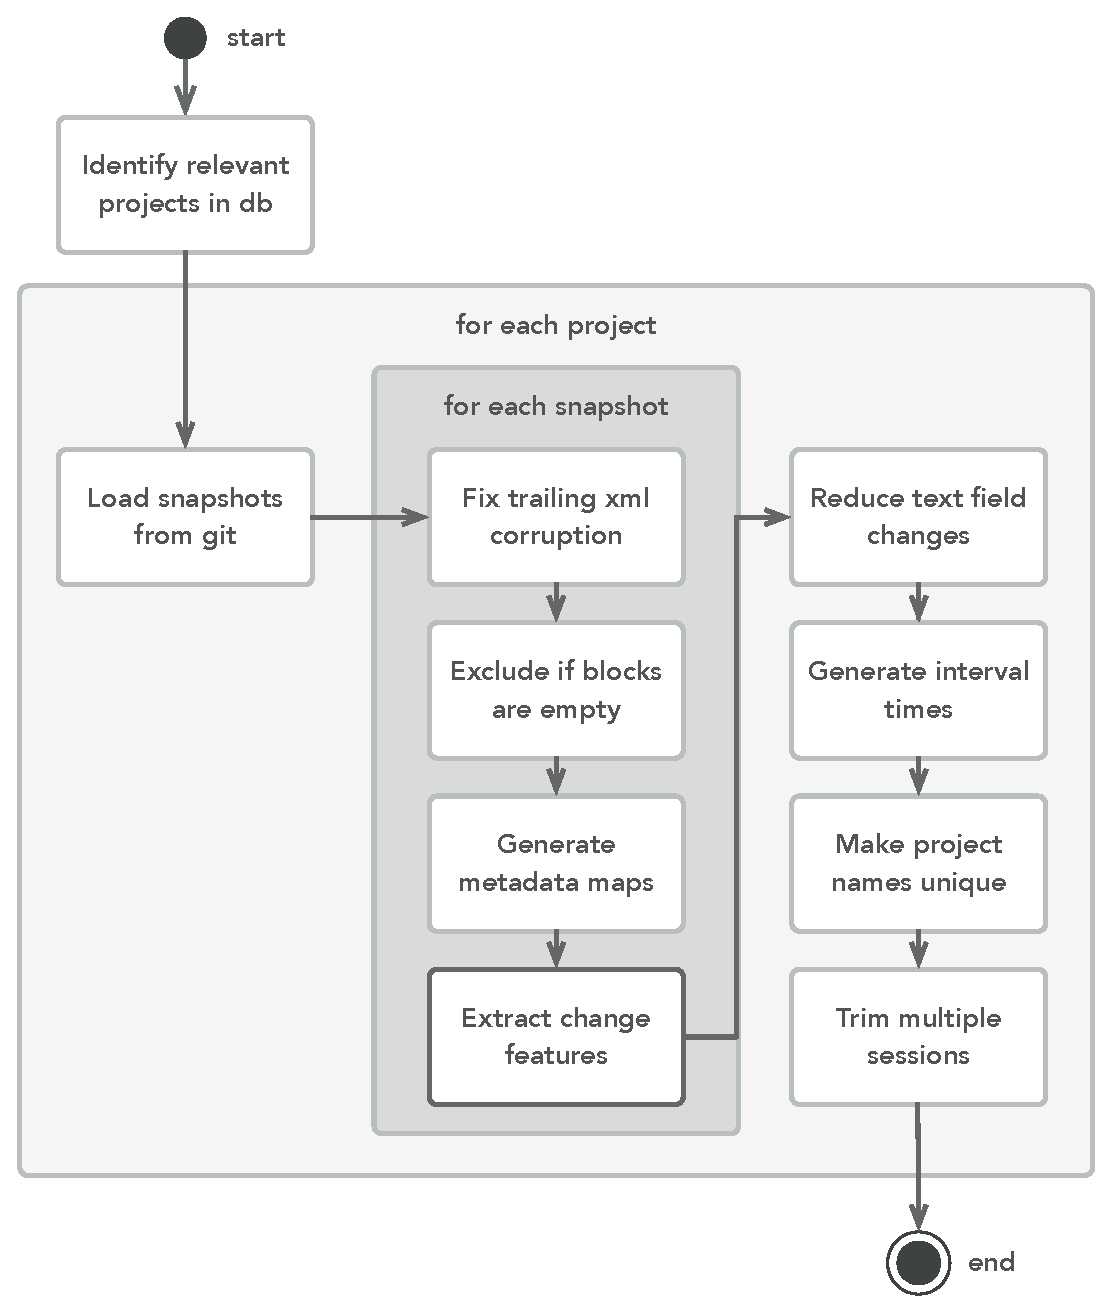
\includegraphics[width=\textwidth]{diagrams/data-import-process}
  \caption[The data importing process]{The data importing process. The entire database was scanned for projects that contain an identifiable element, which were then loaded directly from git. Each change from git was processed for error mitigation and necessary metadata generation, then the features were extracted. After feature extraction, character-wise text field changes were reduced, and then the interval times between snapshots were generated.}
  \label{fig:data-import-process}
\end{figure}

The import pipeline had many tasks to accomplish, starting with identifying the projects that were relevant for analysis. The App Inventor instance that was used for this study was also used for the entirety of the summer camp curricula, so there were many projects captured in the snapshot database that were not part of the activities specific to this study. This was an intentional part of the protocol to make transition easier for the camp students by only having one App Inventor instance with which to interface. The in-class activities were better isolated, so researchers were able to prepare the room in advance to steer the students transparently towards the specialized instance. 

The activities that were part of this study needed to be found in the database. Students had the ability to rename projects at any point, so it was possible (albeit unlikely) that a relevant project could be renamed. Therefore the protocol included a unique element in the projects, a ``magic string'' in a hard-to-find property of the project. The debugging activity and temperature activity each had a unique identifier string, and these strings were included in the starter code that all students were given. These unique elements were then detectable by scanning the files in the git database prior to import. There were instances of students changing the names of the projects, which demonstrated the need of the unique identifier. 

Once a list of projects were identified using their unique elements, those projects were loaded from git into the analysis environment. The git interface opened each project's repository, extracted a list of all commits, and then checked out each commit in turn, capturing the contents of the files for each commit. A commit represented a single snapshot, and the terms ``snapshot'' and ``change'' were used interchangeably to describe the contents of the commit after this stage. 

Each snapshot was checked for corruption at time of import. Following that, two metadata maps were generated for each snapshot: a map of block ID numbers, and a map of block parents. These maps allowed the feature extractor to easily access a block by its ID number (which would require a full tree traversal without), and easily look up the parent of any given block. With the maps generated, the feature extractor would then be able to run. 

After feature extraction, the text field events were reduced (described below), and finally, with the snapshot set complete, interval times between snapshots were generated. At the completion of these stages, the data were ready for analysis, two more steps were first taken. It appeared in data that more than one project was found per user name, possibly due to computer sharing during the summer camp, when a student would do the activity, then switch off with a partner who would then do it for themselves in a fresh copy of the project. To accommodate this, project names had to be made unique, which was accomplished by adding numbers to duplicate user names found in the database. Finally, projects were trimmed to ensure only data from the first session were considered. This condition was rare, and always took the form of a student opening the project the following day, doing nothing, and closing it or switching to another project. These extra snapshots were removed by trimming any snapshots that occurred beyond one hour after the project was initialized. 

Most stages of the import process were additive and non-destructive, so at the conclusion of import each project and snapshot had all of the data available at all previous steps. For instance, the raw block contents were not lost during feature extraction; the list of features were added to the data structure alongside it. 

The following sections delve further into certain components of the import pipeline, and are presented in pipeline order: corruption mitigation, feature extraction, and text field reduction.


\subsection{Corruption Detection and Mitigation}
Some forms of corruption were found in the snapshot data, all concerning the blocks representation. There were four corruption modes, which are explained below, with their respective mitigation strategies.

The first corruption mode was malformed XML files which contained text beyond the closing XML tag. This, of course, crashed the XML parser. Within the debugging activities, only seven snapshots had this malformation, which were corrected by trimming the excess text. It was noteworthy in those cases that the junk excess text was a repetition of the last characters of the file, lends to a hypothesis of the source of the corruption, discussed below.

The second form was rare, where a snapshot had no contents for the blocks file. In the entire collection of debugging activity snapshots ($n = 6890$), only three snapshots had empty blocks. These snapshots were detected during import and were not included in the research data. The overall history of the projects containing these empty snapshots were unaffected. 

Both of these corruptions were indicative of a bug in the extraction of the block data from Blockly in the browser. It was possible that the snapshot mechanism was able to capture the XML file while it was in an inconsistent state, such as mid-write. This bug may be within the Blockly framework itself, and further investigation is recommended before attempting larger-scale deployment of this method.

The two above corruptions were easily mitigated. A third mode of corruption, however, resulted in properly formed XML, but potentially erroneous data. This mode was characterized by multiple changes happening in a single snapshot, which should have been extremely rare, as each snapshot was triggered by an atomic action in the editor. In reality, there was a small amount of caching in the capture mechanism, as discussed in Section \ref{sec:mod-ai}, which may have contributed to this corruption. There was no inherent problem with multiple changes in a single snapshot, if they all occurred within the capture window of that snapshot. In these erroneous cases, one or more actions appeared to be inconsistently represented over time, which caused git and the subsequent analysis tools to do, undo, and redo the same action in very small spans of time, artificially inflating the representation of those events. 

One project was particularly egregious, and showed this corruption in 71 of its 245 commits, rendering nearly a third of its data unreliable. That project was removed, which left only 50 such potential errors in the remainder of the database, many of which were mitigated by text field accumulator, described in Section \ref{sec:text-acc}. 

A data consistency bug was found where a project was opened over more than one session. In App Inventor, if a project was opened in a second, disjoint session, such as the following day, the block ID numbers change, causing the feature extractors to falsely over-report blocks being deleted and added, when really the same blocks have been re-numbered. The strategy employed was to ignore snapshots that occurred at a time stamp beyond the maximum time of the activity.

The total percentage of potentially erroneous snapshots in the debugging activity dataset was 0.84\%. These are summarized in Table \ref{tab:data-corruption}.

% % Debug:		empty blocks - 3 (now, many were hand-fixed, notes may indicate more)
% %				junk past tag - 7 (now, many were hand-fixed, notes may indicate more)
% %			6890 snapshots total
% % Temperature:	empty blocks - 1 
% %				junk past tag - 4 
% %			2296 snapshots total
	
\begin{table}
\begin{centering}
	\begin{tabular}{l r l p{5.4cm}}
	Corruption Mode 		& \multicolumn{2}{l}{Instance Count} 		& Mitigation Strategy 			\\ \hline
	Empty block file 						&  3 &(0.04\%) 				& snapshot deleted 						\\
	Junk beyond \mintinline{xml}|</xml>| 	&  7 &(0.1\%) 				& junk trimmed, snapshot kept 			\\
	Multiple changes 						& 50 &(0.7\%) 				& accepted as insignificant 			\\
	Multi-session 							&  3 &(0.04\%) 				& data past 40 minutes ignored
	\end{tabular}
	\caption[Data corruption modes]{Data corruption modes, their prevalence, and mitigation strategy.}
	\label{tab:data-corruption}
\end{centering}
\end{table}


\subsection{Feature Extractor}
\label{sec:feature-extraction}

\begin{table}
\begin{labeling}{Blocks Moved in Context}

	\item [Blocks Added] Block(s) were added to the workspace. Nearly always a single block.
	\item [Blocks Deleted] Block(s) were removed from the workspace.
	\item [Blocks Moved in Space] Block(s) moved position on the workspace, but did not necessarily change programmatic meaning.
	\item [Blocks Moved in Context] Block(s) changed programmatic position, indicating a new parent block and a different place in the app's control flow.
	\item [Fields Changed] A block's text field changed. Could be a text literal, a variable or procedure name, or a number literal.
	\item [Properties Modified] One or more properties of a block has changed, which could indicate use of the mutator to change a block's semantics (such as changing the number of addends in an addition block). Intended as a catch-all if the other tests missed something, and was rarely found in the data.
	
\end{labeling}
\caption[Features extracted from snapshots]{Features extracted from snapshot data.}
\label{tab:features-extracted}
\end{table}

The features extracted by this module were listed and described above. % in Figure \ref{tab:features-extracted}. 
This section outlines the specific definitions that constitute the feature tests. All of these tests operated on snapshots of the same project that were adjacent in time. 
They detected differences between the two, often utilizing the meta data maps described above in Section \ref{sec:data-processing}. 
% Source code for these algorithms are presented in Appendix \ref{src:feature-extraction-tests}.

The test for \emph{Blocks Added} and \emph{Blocks Deleted} were the same routine, which assembled a list of blocks by their ID numbers for both snapshots and compared differences between those lists using set arithmetic. 

The test for \emph{Blocks Moved in Space} assembled a list of blocks that were present in both snapshots, and iterated that list looking for blocks who were both top-level and whose coordinates changed. There was an important distinction made here- blocks that were nested within other blocks were not top-level and therefore did not trigger the \emph{Blocks Moved in Space} flag when they moved as a consequence of their parent moving. Only blocks whose parent is the workspace itself may return positive from this test, and then, only if they actually moved on the workspace.

\emph{Blocks Moved in Context} was the opposite of the above test, where it detected if a block moved in computational context, indicated by a changed parent. Similarly, this test assembled a list of blocks common to both snapshots, and iterated across that list. The iteration checked if the parent for the block was the same in both snapshots, and returned true if they were not. 

To detect \emph{Fields Changed}, common blocks were listed and then filtered for field properties. Those fields were searched for cases where the value of the fields differed between the two snapshots.

The final test, \emph{Properties Modified} caught any other modifications to a block. This test was more complex. Like those above, it assembled a list of blocks present in both snapshots. It then ran an exhaustive element-wise equality check on each block, comparing the version in each snapshot. If the equality check returned true, that block did not change in any way. If the equality check was false, then lists of all children for both blocks were assembled, which included properties, data fields, mutator instructions, and other Blockly metadata. This step excluded text fields, as they were covered in a previous test. If the lengths of the lists of children were unequal, then the routine returned true, as these particular blocks definitely changed between the two snapshots. If they have the same number of children, then each pair of children were iterated, and the element-wise equal was applied to each of them, effectively running a first-level recursive equality test. If that test did not find any differences, then the routine returned false. That final false return is a condition that should be impossible, but was included defensively, as there may have been edge cases possible in Blockly that were not common in known to the researchers at the time of this design.


\subsection{Text Field Change Accumulator}
\label{sec:text-acc}
In the course of working on their activities, students often manipulated fields of text, including text literals, variable names, procedure names, and parameter names. Examples of blocks utilizing open text fields are shown in Figure \ref{fig:text-fields}. Whenever a text field was modified, the change event was triggered for every character. This was a degree of granularity too fine for meaningful analysis, as character modification events are considered too primitive to be of use \citep{omori2008change}. The snapshot system at runtime could not discern the beginning and end of field editing events, so the change event feature \emph{Fields Changed} from Table \ref{tab:features-extracted} was grossly over-represented. 

To combat this over-representation, sequences of character-wise change events needed to reduced to their final state, which then represented a single change at the same degree of abstraction as the surrounding block manipulations. This reduction was accomplished with an accumulator algorithm, which scanned a project's change history and identified uninterrupted sequences of field modifications to the same field. The algorithm deleted all but the final \emph{Fields Changed} events, leaving only the final state of the modification for further processing. This algorithm had a 10-second timeout, so sequential edits to the same field would be considered different events if there were more than 10 seconds between them. Changes to different field blocks were also considered a new event. This algorithm is shown and further explained in Appendix \ref{src:reduceFieldChanges}.

\begin{figure}
  \centering
      \includegraphics[width=\textwidth]{images/ch4-text-fields}
  \caption[Examples of text fields in App Inventor]{Examples of some text fields in App Inventor. All of the fields, represented by the text in shaded bubbles, could be edited arbitrarily by the student.}
  \label{fig:text-fields}
\end{figure}


\section{Manual Assessment}
\label{sec:manual-assessment}
To get a feel for the data collected, all student projects were inspected by researchers using the snapshot playback mechanism described in Section \ref{sec:playback}. Looking at the students' blocks and their changes over time, researches took note of projects that demonstrated flailing behavior and projects with strong efficacy towards solving the problem. The remaining projects were considered typical. This analysis did not utilize a rubric, nor was intended to be absolute nor complete, as it relied entirely on judgment by the researcher. It did serve to develop an understanding of common patterns, which will be discussed in Section \ref{sec:patterns}. This assessment was necessary to develop the in-depth analysis techniques and visualizations described in sections below. The flailing behaviors were characteristically repetitive, where blocks would move in ways that did not change or improve the state of the app. The high-efficacy behaviors were easier to characterize, as the solution became closer to correct.

In detail, manual assessment rated projects efficacy ``ok,'' ``good,'' ``great,'' or none, and rated repetitive, and/or nonproductive behavior as ``flailing,'' ``extreme flailing,'' ``disengaged,'' ``lacking traction,'' or none. For analysis of these ratings, they were grouped together, where ``good and great'' were a single category, as were all forms of flailing, disengagement, or low traction. All other codes and projects were considered ``typical.'' The counts of these code groups are shown in Table \ref{tab:manual-percentages}.

\begin{table}
\begin{centering}
	\begin{tabular}{l rl rl}
													& \multicolumn{2}{c}{Debugging} & \multicolumn{2}{c}{Temperature}  \\ \hline
		Efficacy ``Good'' or ``Great''				& 31 	& (31\%) 	& 8 	& (29\%) 	\\
		Flailing, Disengaged, or Lacking Traction	& 23 	& (23\%)	& 11 	& (39\%)	\\
		Both of the above							& 4 	& (4\%)		& 1 	& (7\%)		\\
		Uncoded	(typical)							& 52 	& (52\%)	& 11	& (40\%)

	\end{tabular}
	\caption[Coding Results from Manual Assessment of Playback Data]{Coding results from manual assessment of playback data.}
	\label{tab:manual-percentages}
\end{centering}
\end{table}

There was a small sample that was coded for both good efficacy and flailing, totaling four projects over the two activities. These projects showed a degree of flailing followed by correct solutions. These will be explored further in Section \ref{sec:case_analysis}.



\section{The Particle Analysis Method}
\label{sec:particle-analysis}

The purpose of this study was to develop a tool, informed by students' fine-grained programming activities, that can aid a teacher in deciding how to apply their resources during a lab session in real time. A significant insight was reached during analysis of the above change-type features, that such a tool could be constrained to standardized, ``on-rails'' programming assignments. These closed-ended assignments constitute the bulk of many curricula in use, such as those described by  \citet{gray2012teaching}, \citet{martin2015dual}, and \citet{morelli2015analyzing}, and are particularly common at the beginning of curricula, when students are still learning the basics. This situation would be the ideal use case for an orchestration aid. 

With this insight, and the constraint it brought, design began for both a visual tool to help a teacher orchestrate, and an analysis method to power it. The resulting method was \emph{particle analysis,} which borrowed its name from the behavior of atoms and molecules. With this method, a solution to an activity can be regarded as a complex molecule, which was built up out of smaller molecules, which were themselves composed of atoms. In this analogy, every individual block was an atom, and were combined on the workspace to make expressions, representing molecules. A solution to an activity was one or more of these molecules, which could have any number of atoms within them. The analogy could be further extended, admittedly weakly, to correspond the solution to an activity with the chemical definition of ``solution,'' a homogeneous mixture composed of two or more substances. 


\subsection{Features}
Particle analysis offered a number of advantages. It offered an assessment of student progress over time during a programming activity. This metric could easily be charted over time, which created compelling illustrations of that student stories. 

This approach has demonstrated a number of advantages:
\begin{description}
\item [Speed] The algorithm will be implementable on any imaginable platform with real-time performance. 
\item [Breadth] It evaluates blocks even when they are disconnected from executable paths, which contain useful information.
\item [Solution-robustness] It is indicative of progress even if student arrives at a solution that doesn't exactly match the canonical solution.
\item [Problem-robustness] Gift code is accommodated, and with it can show regression below starting point.
\item [Independence] Instructor intervention doesn't affect quality of data, as progress is measured without needing to know where it came from.
\end{description}

\subsection{Definition of Flailing}
With the development of particle analysis, flailing could be formally defined. 
\begin{quote}
\textbf{``Flailing'' is any period of time where changes were made without improvement in the solution particle score.}
\end{quote}
This is different than inactivity, which is a period of time in which no changes were made, which also results in no improvement (or any change) in the particle solution score.

Flailing also includes periods of oscillation, where the score may change often, but does not deviate far from the average over that period, and does not result in an overall improvement of score. 


\subsection{Example}

\begin{figure}
  \centering
      \includegraphics[width=\textwidth]{images/particles-graph-annotated}
  \caption[Solution particle charted scores for two students]{Solution particle charted scores for two students, showcasing insight into their different journeys towards the activity's solution. The vertical bars denote 5-minute periods.}
  \label{fig:paricles-temperature-two}
\end{figure}

The story of two students are charted in Figure \ref{fig:paricles-temperature-two}. This section will now unpack this chart and deduce the stories behind it. These students were working on the Temperature Activity, which was the harder activity, and suffered from a lack of scaffolding before the activity began. This flaw enabled a diversity of behavior patterns to be observed, two of which are depicted here. The horizontal axis is time, and the vertical is their particle score. In this example, a score of 27 was the maximum score for the assignment. The higher the data point is vertically, the closer to the solution the student was. Each mark represents a change within that student's project, and the density of the marks makes for an easy visual indicator of the speed of changes during certain periods. The darker vertical bars delineate 5-minute intervals.

At the beginning of the activity, both students had a period of inactivity (annotation 1), which was likely while instructions were presented to the class. Inactivity is visible as a lack of marks along the line. The student in blue, we'll call Student A, began work at annotation 2, and quickly made some progress. That student then reached a small plateau (3), which included a slight oscillation of score, and a high-density area of changes made without score improvements. This student continued to make generally positive progress, but fell into more high-activity periods without score improvement, at (7) and (8). Additionally, this student had large oscillations in the third period, but not in large jumps. Large jumps of many points in a single change were usually attributed to large assemblies of blocks moving in and out of context together, but this did not appear to be the case between (7) and (8), as there are marks all along the way of the oscillations. Student A completed the activity (9) 14 minutes after starting it, at approximately 16 minutes into the activity. This trajectory is not necessarily bad, but it differs starkly from Student B.

The other student, whom we'll call Student B, began work later at annotation 4, and moved quickly towards the solution. This student progressed largely monotonically, with the exception of one small oscillation (5). The student finished the activity with significant momentum (6), approximately 2 minutes after they began, at approximately 8 minutes into the activity. This trajectory suggested that the student understood the activity fully when they began, and only encountered minor issues. 

We can hypothesize from these trajectories that Student A conducted significantly more experimentation, as their solution score was usually in flux. This student did, however, exhibit periods of rapid changes without a score improvement, which was likely either indicative of flailing or non-functional block re-organization. These possible behaviors, at a glance, represent opposite degrees of concern. If the rapid changes without improvement were flailing, then that student likely required intervention. If the rapid changes were block reorganization, then that student's need for help may depend on the current context, as re-organization could be a disengaged, time-wasting behavior. %TODO I know I have a reference for this.

In this study, interventions from instructors or assistants during the activities were not documented. The lack of intervention data did not affect this analysis, as progress was identifiable regardless of assistance received. This method flipped the problem into an analysis tool, as with it we could make informed guesses as to when assistance took place. In Figure \ref{fig:paricles-temperature-two}, it is likely the student received assistance at annotation 8, and possibly earlier, around annotation 5. 

The only way to know for sure what these specific behaviors mean is to conduct a tightly-controlled experiment where student's real-world behavior is recorded and compared to their solution particle score chart. However, such a study is not necessary to use this analysis method to create a useful teacher-facing tool. Judging the context of student behavior in real-time is a major component of classroom orchestration \citep{dillenbourg2012design}, and a skill in which teachers are specifically trained. Teachers are good at making judgment calls on which students need what, and the particle analysis method can be used to power a tool that can give teachers the information necessary for them to extend their skills into the computer lab. This tool is presented in Section \ref{sec:classroom-console}.


\subsection{How it Works}
This method worked by scanning the entire blocks workspace for individual blocks that were relevant to the canonical solution to the given problem. Each ``atom'' scored a point simply for existing somewhere on the workspace. If that atom was also in its correct location, meaning it had the correct type of block as its parent, an additional point would be added to the score. This technique could be used to nest atoms into others to make code molecules. These molecules could be represented by any number of atoms, which allowed solutions of any degree of complexity to be described.

\begin{figure}
  \centering
      \includegraphics{images/ch4-particle-example-5div}
  \caption[Example blocks to demonstrate nested particle tests]{An example block pattern to demonstrate nested particle tests. The test searches first for the number `5' literal, then whether it is in a division, then whether it is in the correct position of that division.}
  \label{fig:particle-example-5div}
\end{figure}
In its current implementation, up to two additional position tests could be run contingent on the detection of an atom block. Take an example from the Temperature Activity, which requires a number literal to be used as a divisor in a division block. The block combination this example searched for is shown in Figure \ref{fig:particle-example-5div}. The test runner first scans for a number literal block containing the desired value. If it finds one or more of these literals, the first test passes, a point was scored, and it moves to the second test, which queries the location of those found blocks. If any of those blocks were found within a division block, an additional point was scored. The third test operates on the remaining set of number literals inside divisions, and it tested if they were in the correct position in that division, the dividend or divisor. If so, the third point was scored. This process is visualized in Figure \ref{fig:particle-run3}.

\begin{figure}
  \centering
      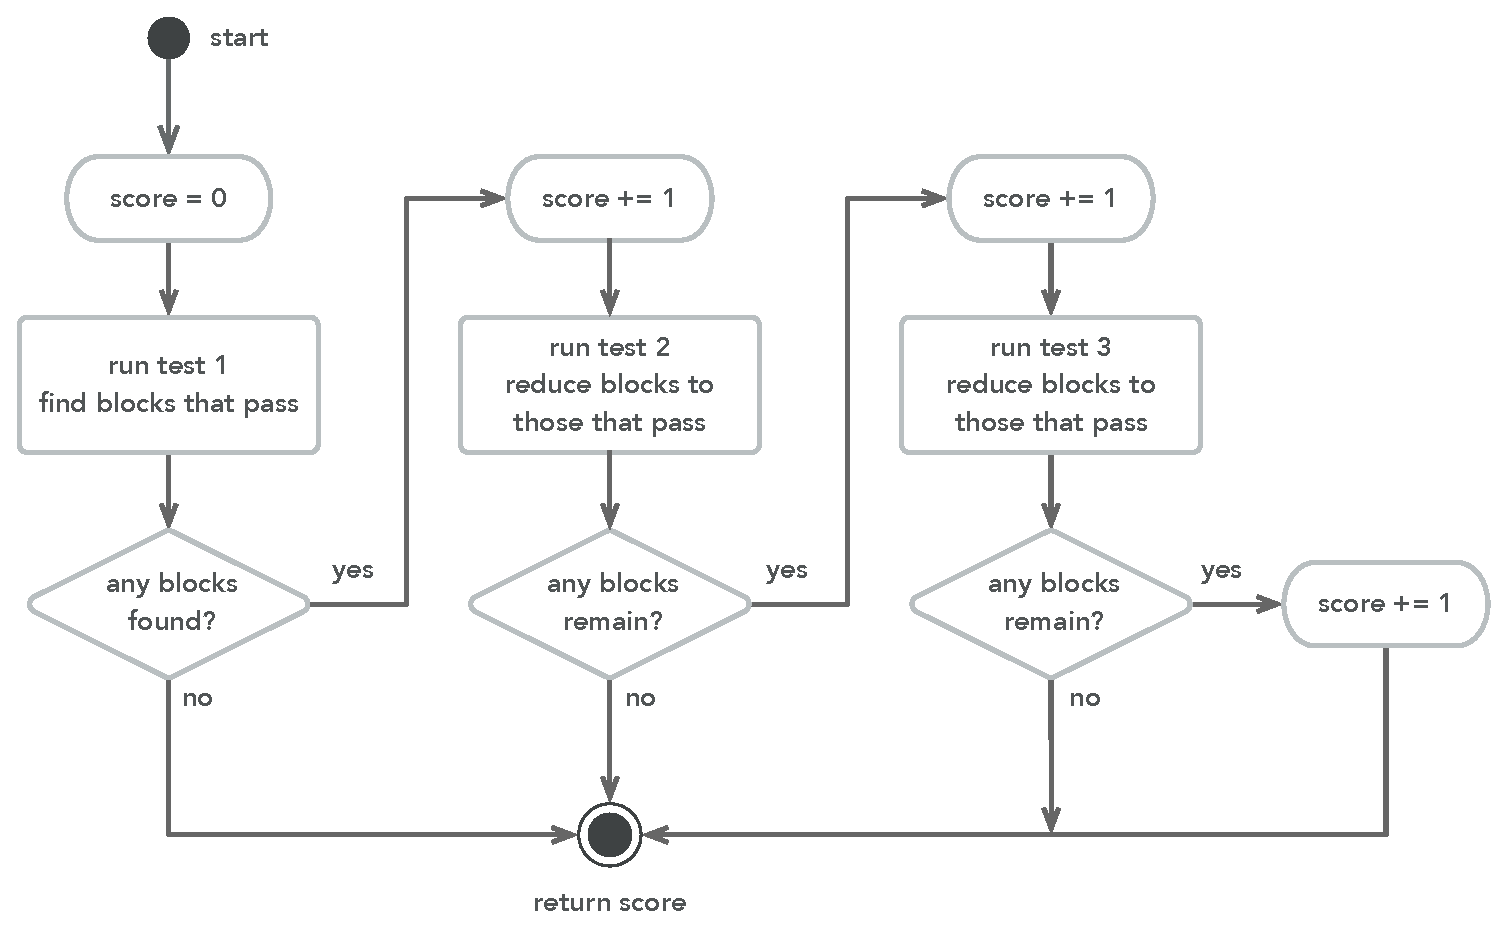
\includegraphics[width=\textwidth]{diagrams/particle-run3}
  \caption[Particle analysis test running algorithm]{Model of the algorithm for running particle analysis tests. This shows the three-test variant. There were also one- and two-test variants, that worked similarly. Test 1 must always be a ``find'' test that looks for individual blocks. Tests 2 and 3 must be ``in a'' tests, which investigate the parent blocks to assess nesting location. 
  %Available tests are listed in Table \ref{tab:particle-tests} in Appendix \ref{app:particle_definitions}.
  }
  \label{fig:particle-run3}
\end{figure}

The tests themselves come in two categories: ``find,'' which looked for certain blocks (the atom finder), and ``in a,'' which tested whether a block was ``in a'' specific parent block type. Additionally, there were helper routines of type ``this is'' which were used by the ``find'' and ``in a'' tests. In Figure \ref{fig:particle-run3}, test 1 must always be of the ``find'' type, and all subsequent tests must be of the ``in a'' type. 

This testing schema included a somewhat nuanced handling of variation, to account for scenarios where students had multiple blocks that satisfied the atom finder. Each test will score a single point if there are one or more blocks that satisfy the test on the workspace. If there are more than one atoms that satisfy a ``find'' test, each subsequent position test would reduce that set. Each test scored as true when the resulting set was non-empty. This method prevents over-rewarding duplicate code by preventing any test from evaluating more than once. Additionally, this provides a reliable maximum score for a given solution definition. This design does not fully handle solution definitions that have repetitive molecules. As an example, if a solution definition were to be written that had two molecules, based on two of the same atom type, but in different locations, it would be possible for a single block to trigger true for both of those ``find'' tests and score two points, which would be a slight over-reward. The over-reward would not persist once the position tests, which must differ, evaluate. This scenario would still render a useful approximation of student progress, though slightly reduced in accuracy. However, if a solution were to call for multiple molecules that evaluate identically, only one implementation would currently be necessary to pass all of those tests. In this scenario, additional differentiating tests would need to be added to the definition, and possibly the evaluation engine, in order to provide a valid progress approximation. 
This logic is also described in Figure \ref{fig:particle-run3}. 

Implementation of these tests varied depending on what properties needed to be evaluated, but they all used helper tools to analyze the XML structure of the blocks workspace. Atom-finding tests were mostly a simple as checking each block for its designating property. Which property needed to be checked varied depending on the type of block, but they were all simple, constant-time reads. The position evaluators (``in a'' tests) were similarly simple, where each block's parent was looked up using the pre-rendered parent mapping structure, and the type of the parent was tested in the same fashion as the ``find'' tests. 

\label{sec:close-enough-text} %this belongs with the paragraph below wherever it ends up
Determining if a text string was equal to the solution's string was less straightforward, as there were many slightly different variations in phrasing that were all conceptually correct. An example was the ``stop shaking me'' text from the Debugging Activity. This string was fed into a text to speech engine to be spoken aloud, so any capitalization or punctuation combination were equally acceptable. Additionally, variations like ``please stop shaking me,'' ``stop shaking me now'' were also conceptually correct. A literal string compare would have regarded those falsely as incorrect. To find strings that were ``close enough'' to the exemplar, a Levenshtein edit distance was used \citep{levenshtein1966binary}. Specifically, what was used was a python implementation of an algorithm proposed by \citet{hyyro2001explaining}, which implemented the Levenshtein distance. To find the acceptable edit distances for ``good enough,'' all strings were collected from all of the activity projects in the database, along with their computed edit distance from their respective exemplar strings. The researchers sorted by edit distance value for each exemplar set, and chose a value which best delineated strings that were variations from those that were wrong. The values were different for the two exemplars: ``stop shaking me'' required an edit distance less than 9, and ``how are you'' required an edit distance less than 4. This process would need to be improved for teachers or curriculum developers to implement their own particle definitions. The method used by the researchers to reach their desired threshold values could be automated using hidden Markov Models, where ``close enough'' and ``not close enough'' examples provided by the user could automatically be assessed for a reasonable threshold value.

The test definitions used in this study are presented in Appendix \ref{app:particle_definitions}. 

\subsection{Current Weaknesses}
The particle analysis method relied on a known solution, and provided a metric of how close to that solution a student was at any time. This was conceptually similar to \citet{le2007using} and \citet{mitrovic2003intelligent}, where both used a pre-made definition of the solution for a particular problem. The particle analysis method also shares a core weakness with those systems, where the solution definitions must be known and written in advance. Adding to the cannon of activities that can utilize the system depends on writing new solution definitions, which may be difficult for in-service teachers who already suffer from limited prep time. Perhaps content authors would be responsible for also including suitable solution definitions, but a fully automated path would clearly be better.

The current implementation of particle analysis allows for a class of solution over-representation, where students can create invalid code that generates a score \emph{slightly higher} than that of the equivalent working code. This bug stems from a language feature of App Inventor that the particle implementation does not yet handle. This class of bug, however, should be directly addressed in the conceptual design of the particle analysis method.


\section{Patterns Observed in Particle Scores}
\label{sec:patterns}

\begin{figure}
	\centering
	\includegraphics[width=\textwidth]{images/stories/scores-debug-UfaDogfish}
	\caption[Smooth, Rapid Progress of Particle Scores]{Smooth, rapid progress of particle scores, as shown by the student UfaDogfish in the Debugging Activity.}
	\label{fig:smooth_chart}
\end{figure}
Across both activities, three general patterns of particle score progression emerged. The first, called ``smooth'' was a rapid acceleration to the conclusion, where nearly every change improved the score. The ``smooth'' category looks like as if the student already knew the answer, and implemented directly and efficiently. This pattern did allow for slight variation, and smooth-coded projects were not always monotonically increasing, but they were always rapid rises with few changes before the beginning of the upward inflection. An example is shown in Figure \ref{fig:smooth_chart}. Less than a quarter (22\%) of Debugging Activity projects showed this pattern, and just over a quarter (27\%) of the Temperature activity did.

\begin{figure}
	\centering
	\begin{subfigure}{\textwidth}
		\includegraphics[width=\textwidth]{images/stories/scores-temp-HangzhouTurkey}
		\caption{HangzhouTurkey in the Temperature Activity}
	\end{subfigure}\hfill
	\begin{subfigure}{\textwidth}
		\includegraphics[width=\textwidth]{images/stories/scores-debug-LondonDragonfly}
		\caption{LondonDragonfly in the Debugging Activity}
	\end{subfigure}\hfill
	\caption[``Fits and Starts,'' Typical Progress of Particle Scores]{Two examples of ``Fits and starts,'' demonstrating the typical progress of particle scores.}
	\label{fig:fits_starts_chart}
\end{figure}
The second pattern category was called ``fits and starts'' and represents the most typical trajectory, where the score has periods of progress, non-progress, and sometimes regression, but overall trends upwards and reaches a reasonably successful final state. This was the most broad category, as it was also the one to catch any pattern that was not clearly smooth (above) or flailing (below). Two examples are provided in Figure \ref{fig:fits_starts_chart}, to show the core pattern and some of the allowable variation around it. The Debugging Activity and Temperature Activity projects fell into this category at rates of 49\% and 60\%, respectively. 


\begin{figure}
	\centering
	\includegraphics[width=\textwidth]{images/stories/scores-debug-RomePelican}
	\caption[Flailing Pattern, a Lack of Progress of Particle Scores]{Flailing pattern is indicated by a lack of overall progress of particle scores, as shown by the student RomePelican in the Debugging Activity.}
	\label{fig:flailing_chart}
\end{figure}
The third pattern category was ``flailing.'' While the ``fits and starts'' category did allow some flailing behavior, whether score oscillation or non-progress changes, that category always had a generally upwards trend, and resulted in a solution. This category of flailing was reserved for the projects that demonstrated little progress in total, and were entirely flailing behaviors. This pattern is shown in Figure \ref{fig:flailing_chart}. 

A proportion (30\%) of the Debugging Activity projects fell into this category, but, surprisingly, only 13\% of Temperature Activity projects did. We had hypothesized that where the Temperature Activity lacked proper scaffolding there would be more flailing behavior, but the largest category was by far ``fits and starts.'' We can posit that the low rate of apparent flailing at this scale may be due to the aggressive availability of helpers for intervention. The problem may have been sufficiently hard that many students did not even try until they got help from someone. This hypothesis is supported by the wide variation of inflection point, the time where the scores began to increase. Some started right away, while others started nearly at the end of the session period, with many in between. This time translation may be an artifact of the teaching assistants working their way through the classroom, eventually giving everyone the intervention necessary for them to understand and be effective within the problem.

These categories, and the students in each for both activities, is shown in Tables \ref{tab:pattern_names_debug} and \ref{tab:pattern_names_temp}.

\begin{table}
\begin{centering}
	\begin{tabular}{p{\textwidth}}
	\hline \hline
	``Smooth'' (23, 22\%)\\ \hline
		CampoPrairie		
		CiudadWeasel		
		CuiabáGoldfish		
		DetroitShark		
		DortmundBat			
		GorakhpurYak		
		GuayaquilRook		
		HamamatsuFrog		
		JohorGuineaPig		
		KermanshahCockroach1
		LagosRook			
		LibrevilleCrow		
		MendozaAnteater		
		ParisAlligator1		
		PeshawarGnat		
		RangoonBear			
		SantaGrasshopper	
		SeoulOkapi			
		TrujilloLouse		
		TurinFly			
		UfaDogfish			
		VisakhapatnamSheep	
		ZaporizhzhyaFalcon	\\ \hline \hline

	``Fits and Starts'' (51, 49\%)\\ \hline
		AcapulcoDeer		
		CairoCat			
		ChelyabinskSpider	
		ConakryBear		
		CórdobaSalmon	
		DatongPigeon		
		DenverDolphin		
		DhakaClam			
		DhakaEchidna		
		DublinBee			
		FukuokaGoldfinch	
		GuayaquilRook1	
		HangzhouTurkey	
		HangzhouTurkey1	
		HefeiKudu			
		HermosilloSandpiper
		HubliMarten		
		IndoreDogfish		
		IndoreWallaby		
		JinzhouGorilla	
		KaohsiungViper	
		KitakyushuSeal	
		KobeCaterpillar	
		KobeSalamander		
		KuchingCheetah		
		LahoreLapwing		
		LondonDragonfly		
		LusakaOx			
		MoreliaOx			
		MultanFrog			
		MunichTermite		
		NanchangOwl			
		OnitshaWombat
		PermHerring
		PhoenixWeasel
		PointeCheetah
		PueblaVulture
		SeoulSheep
		ShahChinchilla
		SholapurSandpiper
		SurabayaChimpanzee
		TaichungRook
		TaizhouSwallow
		TbilisiKudu
		TijuanaOctopus
		VladivostokCurlew
		WarangalStinkbug
		WroclawRat
		XianAntelope
		YanchengGoose
		ZhangjiakouSardine		\\ \hline \hline
	``Flailing'' (31, 30\%)\\ \hline
		CalgaryHyena
		ChongjuOwl
		HachiojiPeafowl
		HamadanMouse
		HaoraDragonfly
		KadunaAlpaca
		KermanshahCockroach
		KhabarovskBoar
		MakhachkalaWasp
		MultanVulture
		NagpurAlpaca
		NiyalaAlligator
		OkayamaMarten
		OklahomaGiant
		ParisAlligator
		PhiladelphiaWoodpecker
		QuerétaroMule
		QuitoShark
		RomePelican
		SapporoWoodcock
		SarajevoDuck
		SurabayaTermite
		SuwonGoldfish
		TaiyuanDinosaur
		TianjinAlbatross
		TripoliSandpiper
		ValenciaFox
		VijayawadaOtter
		WarsawCrocodile
		XuzhouLoris
		YaroslavlCattle	\\ \hline

	\end{tabular}
	\caption[Categories of Progress Patterns for the Debugging Activity and the Students in them]{Categories of Progress Patterns for the Debugging Activity and the Students in them.}
	\label{tab:pattern_names_debug}
\end{centering}
\end{table}

\begin{table}
\begin{centering}
	\begin{tabular}{p{\textwidth}}
	\hline \hline
	``Smooth'' (8, 27\%)\\ \hline
		DortmundBat
		HubliMarten
		KermanshahCockroach
		MendozaAnteater
		RangoonBear
		TbilisiKudu
		UfaDogfish
		ZaporizhzhyaFalcon
		\\ \hline \hline
	``Fits and Starts'' (18, 60\%)\\ \hline
		DatongPigeon
		FukuokaGoldfinch
		HangzhouTurkey
		KobeSalamander
		LondonDragonfly
		PhoenixWeasel
		PointeCheetah
		PueblaVulture
		QuerétaroMule
		ShiheziBat
		SurabayaChimpanzee
		SurabayaTermite1
		TaiyuanDinosaur
		TaizhouSwallow
		VeracruzDotterel
		VisakhapatnamSheep1
		VladivostokCurlew
		WroclawRat
		\\ \hline \hline
	``Flailing'' (4, 13\%)\\ \hline
		Rostov-na-DonuLapwing
		Rostov-na-DonuLapwing1
		SurabayaTermite
		VaranasiOstrich
		\\ \hline

	\end{tabular}
	\caption[Categories of Progress Patterns for the Temperature Activity and the Students in them]{Categories of Progress Patterns for the Temperature Activity and the Students in them.}
	\label{tab:pattern_names_temp}
\end{centering}
\end{table}



\section{The Flailing Detector Algorithm}
\label{sec:the-flailing-detector}
The Flailing Detector Algorithm accepted as input a series of changes represented as particle scores, and assessed each change as flailing or non-flailing based on the scores of the immediately preceding changes. This algorithm is the literal realization of the thesis question specified in Section \ref{sec:problem-statement}. 

The algorithm also takes a parameter as input to specify the number of predecessor changes to examine when assessing for flailing. This parameter was called the \emph{changeWindow}, and was completely independent of time. The changeWindow parameter affected how many changes would be considered, completely irrespective to the time period over which those changes took place. This disregard for time was intentional to create the simplest realization of the Flailing Detector.

For each change, the previous \emph{changeWindow} scores were averaged. If the current change score was greater than the average of its immediate predecessors, that change was marked as non-flailing, otherwise it was marked as flailing. The flailing detector algorithm can be stated as: 

\[F(S_n) = S_n \leq M(S_{n-1} \dots S_{n-w})\]

where $F(s)$ is the Flailing function that returns true to indicate flailing, $S$ is the particle score of a snapshot, $M$ is the arithmetic mean function, and $w$ is the \emph{changeWindow} parameter. 

This definition only works when $n > w$, otherwise $F$ returns false, for non-flailing. This caveat accounts for the startup time necessary to fill the change window. There is no way to know if a student is flailing on the first snapshot alone, and likely not the second. Only once a sufficient number of snapshots are collected ($n>w$) can a flailing assessment be made.

Full source code is listed in Appendix \ref{src:flailing-detector-algorithm}.

\subsection{Argument for Real-time}
The flailing detector algorithm is of time complexity $O(n)$. In detail, it currently is built out of three functions: a one-point calculator, a scanner for an entire project, and an entry point that is a wrapper around the scanner. The wrapper does nothing but sanity check the project type and reformat the data structure, which are both constant-time operations. It then calls the scanner, which uses a for-loop over the length of the project ($O(n)$). In this loop, the one-point calculator is called, which computes the average for the change window (parameter $w$), and compares that average to the current score. The comparison is constant time, and the change window average is $O(w)$. The window parameter $w$ is both small and constant, so the total time complexity of the one-point calculator is constant. The only non-constant operation is the iteration over the project's list of data, resulting in total complexity for the algorithm of $O(n)$, where $n$ is the number of snapshots to be analyzed. This assumes that the particle scores are previously calculated. These complexities would add, not multiply, so the true cost of scanning a series of snapshots would be the cost of calculating the particle score or the $O(n)$ cost of detecting flailing, whichever would be greater.

This assessment is only valid for the post-hoc scanner implementation. A truly real-time solution would not have an array of snapshots to iterate over, rather it would assess flailing as the snapshots were generated. This makes the time spent \emph{per snapshot} most important. As the student works, each change made would be accompanied by a calculation of the particle score followed by the flailing detector calculation. Like the post-hoc implementation above, the time complexities of computing scores and flailing would add, not multiply, so the complexity class would be the greater of the two. 

The calculation of particle scores depends on the definition of the solution, and the number of particles defined in it. Each particle can contain one to three tests, or more, with each test operating on a successively smaller subset of blocks. The driving factor of time complexity are the ``find'' tests, which need to execute a workspace-wide search for blocks of a specific type, and of which there are at most one per particle definition. These tests are currently implemented as linear searches, with time complexity of $O(n)$, where $n$ is the number of blocks in the project. 

Additional optimizations could be made to the real-time version of the particle score assessor to reduce the time of the initial block search. By adding an indexed data structure to track blocks by type, that search could be implemented as a search tree, which would reduce the complexity to $\Theta(logn)$. The flailing detector would only operate on the most recent $w$ data points, so each change would be constant-time, described by the window parameter $w$. The ideal total time complexity would then be $\Theta(logn) + O(w) \in \Theta(logn)$. A less-optimized solution which closer resembles the current working implementation would be $O(n) + O(w) \in O(n)$.



\section{Validation}
Additional post-hoc studies were conducted to validate the tools presented in this chapter. The argument can be summarized:
\begin{description}
\item A. Blocks playback was a suitable tool for manually assessing the presence of flailing behavior in projects (Section \ref{sec:manual-assessment}). 
\item B. Particle Score charts were as good as (A) for manually assessing the presence of flailing within student projects (Section \ref{sec:validation-particle}).
\item C. (B) implies that Particle Scores contain necessary data for the assessment of flailing
\item D. The Flailing Detector Algorithm was effective for automatically assessing the presence of flailing behavior \emph{per snapshot} (Section \ref{sec:validation-flailing-detector}).
\end{description}

\subsection{Particle Analysis for Improved Assessment of Flailing}
\label{sec:validation-particle}
When manually coding for flailing behaviors in a project, one technique was to use the blocks playback mechanism to replay the entirety of the project, in full detail, to view the project's development similarly as if observed over the student's shoulder. This method, while providing the most possible information to the assessor, was time-consuming, and required days to encode a single classroom of data. The Particle Analysis method may be used as a feature extractor, to distill these data into a more succinct form, that still supply information necessary to manually assess for flailing. 

The protocol to manually assess particle scores for flailing involved reading the scores in chart form, such as Figures \ref{fig:smooth_chart}, \ref{fig:fits_starts_chart}, or \ref{fig:flailing_chart}. Each project was coded according to the patterns described in Section \ref{sec:patterns}: \emph{smooth}, \emph{fits and starts}, or \emph{flailing.} These codes conceptually mapped closely to the codes from the earlier playback analysis: \emph{good/great}, \emph{typical/none}, and \emph{flailing.}
These codes were then compared with the similar codes found from the manual assessment of blocks playback data using a Chi-Square test of independence.

The Chi-Square test was selected as it can determine relation between categorical variables, which both coding sets were. The requirements for this test were met with two categorical variables (playback-derived codes and particle-score-derived codes), two or more categories for each variable, and independence of observations. The null hypothesis ($H_0$) stated that the variable 1, playback-derived codes, were independent or variable 2, the particle-score-derived codes. The alternative hypothesis ($H_1$) was the opposite, and stated that the the variables were related.

The test had $n=138$ projects. The crosstabs table of this test is shown in Table \ref{tab:crosstab-blocks-particle}.
\begin{table}
\begin{centering}
	\begin{tabular}{l l r r r | r}
			&& \multicolumn{3}{c}{Particle-derived Codes} 	\\
			&	& flail 	& smooth 	& fits and starts 	& total	\\ \hline
	\multirow{3}{*}{Playback-derived Codes}
	& flailing 		& 17	& 2			& 11		& 30	\\
	& good/great	& 3		& 19		& 16		& 38	\\
	& typical/none	& 18	& 10		& 42		& 70	\\ \hline
	total	&  		& 38	& 31		& 69		& 138
	\end{tabular}
	\caption[Flailing crosstabs between Blocks Playback and Particle Scores]{Crosstabs between Blocks Playback and Particle Score codes for flailing within a project.}
	\label{tab:crosstab-blocks-particle}
\end{centering}
\end{table}

The Chi Squared test returned a Pearson coefficient of 35.837, with no cells having fewer counts than expected. With 4 degrees of freedom, the asymptotic significance was $p<.001$. We rejected the null hypothesis, and we concluded that there was a significant association between the coding set derived from blocks playback and the coding set derived from reading particle score charts ($\chi^2(4)> = 35.837$, $p < .001$). 


\subsection{Validating the Flailing Detector}
\label{sec:validation-flailing-detector}
In the previous sections, the analysis techniques categorized entire projects by the degree of the flailing they contained. That method is different than the actual goal of the flailing detector, which needs to operate in real-time, evaluating the data as it generated. This change-by-change assessment must work without the benefit of the entire project's vector for context. To validate this type of data, a portion of the database were manually assessed by researchers for flailing on a point-by-point basis, by evaluating periods of flailing, noting their start and end points, and filling the ranges of points with the flailing or non-flailing. The result was a new data set where each change was marked as flailing or not by a researcher, and this set was compared to the results of the same data as processed by the flailing detector algorithm. 

The data collected from the study contained 8,778 unique data points, where each point was a change made to a project. These points were across 138 projects, including both the Debugging and Temperature activities. A validation subset for manual assessment was randomly selected to represent 10\% of the total data. The procedure for this selection to randomly select a project, and add its changes to the selection. Additional projects were randomly selected until the number of changes in the selected projects was greater than or equal to 10\% of the total change count. The final validation subset contained 16 projects, listed in Table \ref{tab:selected-projects}, representing 881 changes, which was 10.03\% of the total data collected.

\begin{table}
\begin{centering}
\begin{tabular}{l l r}
	Activity & Code Name & Change Count \\ \hline
	debugging & AcapulcoDeer & 44\\
	debugging & CórdobaSalmon & 132\\
	debugging & HachiojiPeafowl & 48\\
	debugging & HamamatsuFrog & 9\\
	debugging & JinzhouGorilla & 61\\
	debugging & NagpurAlpaca & 8\\
	debugging & PeshawarGnat & 12\\
	debugging & PointeCheetah & 95\\
	debugging & PueblaVulture & 40\\
	debugging & XuzhouLoris & 25 \\
	temperature & DortmundBat & 64\\
	temperature & FukuokaGoldfinch & 70 \\
	temperature & LondonDragonfly & 99 \\
	temperature & UfaDogfish & 42\\
	temperature & VladivostokCurlew & 90 \\
	temperature & ZaporizhzhyaFalcon & 42 \\ \hline
	\multicolumn{2}{r}{Total} & 881
\end{tabular}
\caption[Projects and Change Counts Selected for the Validation Data Set]{Projects and change counts selected for the validation data set, which represented 10.03\% of the database, as counted by individual changes.}
\label{tab:selected-projects}
\end{centering}
\end{table}

The Flailing Detector algorithm was applied to the same projects in the validation selection with a change window parameter of 5. There were two coded data sets for comparison, both generated from the source data. The first set was the human-coded flailing and the second, the automatically generated flailing codes from the algorithm. These sets were tested using the Chi-Square Test of Independence, similarly to the particle assessment test in Section \ref{sec:validation-particle}.

The Chi Squared test was selected as it can determine relation between categorical variables. The requirements for this test were met with two categorical variables (flailing per point, from two sources), two or more categories for each variable (flailing, non-flailing), and independence of observations. The null hypothesis ($H_0$) stated that the variable 1, the manually assessed codes, were independent or variable 2, the automatically assessed codes. The alternative hypothesis ($H_1$) was the opposite, and stated that the the variables were related.

The test had $n=881$ changes (points). The crosstabs table of this test is shown in Table \ref{tab:crosstab-flailing-detector}.
\begin{table}
\begin{centering}
	\begin{tabular}{l l r r | r}
			&& \multicolumn{3}{c}{Automatic Codes} 	\\
			&	& Flailing 	& Non-Flailing 	& total	\\ \hline
	\multirow{2}{*}{Manual Codes}
	& Flailing 		& 421	& 161		& 582	\\
	& Non-Flailing	& 42	& 257		& 299	\\ \hline
	total	&  		& 463	& 418		& 881
	\end{tabular}
	\caption[Flailing Crosstabs for Flailing Detector Validation]{Crosstabs between manually assessed and automatically assessed flailing on the same data, to validate the flailing detector algorithm as similarly effective as manual interpretation.}
	\label{tab:crosstab-flailing-detector}
\end{centering}
\end{table}

The Chi Squared test returned a Pearson coefficient of 269.154, with no cells having fewer counts than expected. With 2 degrees of freedom, the asymptotic significance and Fisher's Exact Test significance were both $p<.001$. We rejected the null hypothesis, we concluded that there was a significant association between the manually-assessed and automatically-generated flailing codings, which validated the Flailing Detector Algorithm ($\chi^2(2)>= 269$, $p < .001$). 





\section{The Classroom Console}
\label{sec:classroom-console}

\begin{figure}
  \centering
      \includegraphics{images/ch4-console-demo}
  \caption[Excerpt of the Classroom Console]{An excerpt of the Classroom Console visualization, showing three students.}
  \label{fig:console-demo}
\end{figure}


Based on the insights afforded by the particle analysis method, an orchestration technology was designed. Orchestration, as \citeauthor{dillenbourg2012design} described, ``refers to how a teacher manages in real-time multi-layered activities in a multi-constraints context" (\citeyear{dillenbourg2012design}). In the general case of App Inventor classrooms, teachers need to manage many levels of technology in addition to the difficult task of managing class-wide pedagogy, and the scaffolding of specific students as necessary. The orchestration technology developed here aims to support the activity of orchestrating \citep{tchounikine2013clarifying}.

The orchestration technology is referred to as the Classroom Console. An excerpt of the console is shown in Figure \ref{fig:console-demo}. This console, at a glance, gives teachers insight into the status of individual students and the class as a whole. Multiple dimensions of information are presented with visualization strategies that we believe are aggregated to a degree that makes it useful lightweight to use. The goals of the console are follows, for each student, it must display:

\begin{description}
\item [Current particle score] The primary display element is the student's current score. This is updated in real-time as they work.
\item [Time since score advanced] A ``timeout bar'' accompanies the score display, showing how much time has elapsed since the score has increased.
\item [Active or away] The timeout bar changes color to indicate whether the student is working actively or idle.
\end{description}

Additionally, the console must give the teacher a ``landscape view'' of the entire class. The visual score bars for each student are easily assessed as a group, so approximate progress of the entire class can be seen at a glance. If all the bars are low, then the class in general is either at the beginning, or may be in need of a class-wide clarification or hint. 

\subsection{Pre-Recorded Data}
This tool was a conceptual mockup. It did not work with live-collected data, but did operate on previously collected data from the study. The console as seen here is effectively a replay device, playing back real classroom data that were collected in real time. The data were genuine, and the timings expressed were the real-time observations of real students in their environments. This platform is ideal for design discussion. Connecting this concept to a live learning management environment is reserved for future work. 

\subsection{The Console in Detail}
A single student's display is annotated in Figure \ref{fig:console-single-annotated}. It shows the student's identifier, which could be their name (a), their current score on the problem from particle analysis (b), and a timeout bar (c). The timeout bar fills in one-minute intervals, starting with zero. The timeout bar also changes color to reflect when the student is no longer actively working, and has become idle. This ``away'' indicator can be seen in Figure \ref{fig:console-demo}, where the first two students are active and the third is away. The third student's idle bar is a lighter color.

A full classroom of 29 students is shown in Figure {fig:console-classroom}. There are many stories that can be deduced from this single moment. At the time of capture, many students had completed or near-completed the activity, indicated by the prevalence of tall blue bars. Students KermanshahCo, KobeSalamander, and PhoenixWeasel were examples of students who had completed the activity, and then became idle. Logically, at the conclusion of the activity these students became idle, as they had nothing left to do. They may have been elsewhere in the classroom, but were no longer engaging with App Inventor. Conversely, TaizhouSwallow, located in the lower-left corner of the Console, appeared to be having difficulty. This student is showing a low score, and has also been actively working with no forward progress for five minutes or more. Students with no indicators in the timeout bar, such as PointeCheetah and ShiheziBat in the middle row, had progressed their scores forward within the last minute. Every block in the timeout bar represented one minute of time, and a full bar of five blocks indicated five or more minutes without progress. 

\begin{figure}
  \centering
      \includegraphics{images/ch4-console-single-annotated}
  \caption[One student display, annotated]{One student's display from the Classroom Console. }
  \label{fig:console-single-annotated}
\end{figure}


\begin{figure}
  \centering
      \includegraphics[width=\textwidth]{images/ch4-console-class}
  \caption[Full classroom display of the Classroom Console]{A full classroom of 29 displayed in the Classroom Console.}
  \label{fig:console-classroom}
\end{figure}

